%%%%%%%%%%%%%%%%%%%%%%%%%%%%%%%%%%%%% 
%% LE2I beamer template
%% Guillaume Lemaitre, October 2014
%%%%%%%%%%%%%%%%%%%%%%%%%%%%%%%%%%%%% 

\documentclass{beamer}

\usepackage[utf8]{inputenc}
\usepackage[T1]{fontenc} 
\usetheme{le2i} 

%% The amssymb package provides various useful mathematical symbols
\usepackage{amssymb}
%% The amsthm package provides extended theorem environments
\usepackage{amsthm}
%% amsmath for math environment
\usepackage{amsmath}

\DeclareMathOperator*{\argmin}{arg\,min}
\DeclareMathOperator*{\argmax}{arg\,max}
\DeclareMathOperator*{\sign}{sign}

%% figure package
\usepackage{epsf,graphicx}
\usepackage{epstopdf}
\usepackage{subfigure}
\usepackage{transparent}

%% In order to draw some graphs
\usepackage{tikz,xifthen}
\usepackage{tikz-qtree}
\usepackage{adjustbox}
\usetikzlibrary{decorations.pathmorphing}
\usetikzlibrary{fit}
\usetikzlibrary{backgrounds}
\usetikzlibrary{shapes,arrows,shadows}
\usetikzlibrary{calc,decorations.pathreplacing,decorations.markings,positioning}
\usetikzlibrary{snakes,decorations.text,shapes,patterns}
% \usepackage{scalefnt,lmodern,booktabs}

%% Package for cross and tick symbols
\usepackage{pifont}
\newcommand{\tick}{\color{green!60!black!80}\ding{51}}
\newcommand{\cross}{\color{red!60!black!80}\ding{55}}

\title{RE-COOP \#8: \\ \  \\ {\Large A round-up around GIT ... \\ ... informal of course !!!}}
\author{Cedric Lema\^itre \\ Guillaume Lema\^itre \\ Joan Massich}
\date{16\textsuperscript{th} September 2020}

\institute{Universitat de Girona, Universit\'e de Bourgogne} 

%% Uncomment if you want to avoid thousand of bullet inside the menu
% \usepackage{etoolbox}
% \makeatletter
% \patchcmd{\slideentry}{\advance\beamer@xpos by1\relax}{}{}{}
% \def\beamer@subsectionentry#1#2#3#4#5{\advance\beamer@xpos by1\relax}%
% \makeatother

\begin{document}

% Show the title page
\begin{frame}
  \titlepage
\end{frame}

% Show the table of contents
\begin{frame}[shrink=40]
  \vspace{40px}
  \tableofcontents[sectionstyle=show,subsectionstyle=show,subsubsectionstyle=hide]
\end{frame}

\section{History}

%\subsection{First subsection}

\begin{frame}
  \frametitle{A bit of History ...}
  %\framesubtitle{A Kick-Ass Title Subtitle}
  \begin{block}{For Microsoft Windows users}
    \begin{figure}
      \centering
      \includegraphics[width=.2\textwidth]{./images/git-logo.png}
    \end{figure}
    \begin{figure}
      \centering
      \includegraphics[width=.6\textwidth]{./images/git-windows.png}
    \end{figure}
  \end{block}
\end{frame}

\begin{frame}
  \frametitle{A bit of History ...}
  \begin{block}{For Linux users}
    \begin{figure}
      \centering
      \includegraphics[width=.35\textwidth]{./images/git-mess.png}
    \end{figure}
  \end{block}
\end{frame}

\begin{frame}
  \frametitle{A bit of History ...}
  \framesubtitle{Original author}
  \pause
  \begin{block}{Linus Torvalds}
    \begin{figure}
      \centering
      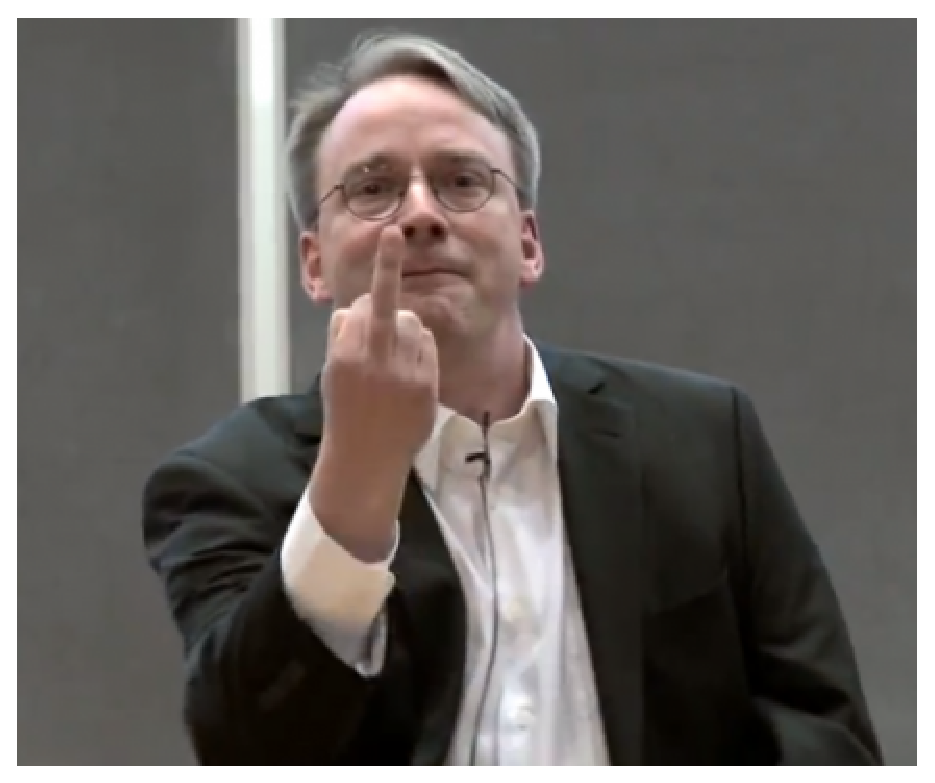
\includegraphics[width=.5\textwidth]{./images/linus.eps}
    \end{figure}
  \end{block}
\end{frame}

\section{What is GIT?}

\subsection{Definitions}

\begin{frame}
  \frametitle{What is GIT?}
  \framesubtitle{Definitions}
  \begin{block}{\small Formal definition}\footnotesize
    \begin{itemize}
    \item Git is a distributed revision control system with an emphasis on speed, data integrity, and support for distributed, non-linear workflows. 
    \item Since 2005, it has become the most widely adopted version control system for software development.
    \end{itemize}
  \end{block}
  \pause
  \begin{block}{\small In an everyday language}\footnotesize
    \begin{itemize}
    \item THIS IS COOL AND FANCY!!!!
      \pause
    \item[\tick] Keep track of all changes performed on a repository,
      \pause
    \item[\tick] Allow to have multiple versions,
      \pause
    \item[\tick] Possibility to swap versions,
      \pause
    \item[\tick] Perform collaborative work,
      \pause
    \item[\tick] Easy way to merge work,
      \pause
    \item[\cross] Need to learn the tool.
    \end{itemize}
  \end{block}
\end{frame}

\subsection{1$^{st}$ study case}

\begin{frame}
  \frametitle{What is GIT?}
  \framesubtitle{Study cases}
  \begin{block}{Software versioning}
    \begin{figure}
      \centering
      \includegraphics[width=.5\textwidth]{./images/brick.png}
    \end{figure}
  \end{block}
\end{frame}

\subsection{2$^{nd}$ study case}

\begin{frame}
  \frametitle{What is GIT?}
  \framesubtitle{Study cases}
  \begin{block}{Student case}
    \begin{figure}
      \centering
      \includegraphics[width=.7\textwidth]{./images/coding.png}
    \end{figure}
  \end{block}
\end{frame}

\subsection{3$^{rd}$ study case}

\begin{frame}
  \frametitle{What is GIT?}
  \framesubtitle{Study cases}
  \begin{block}{Writing case}
    \begin{figure}
      \centering
      \includegraphics[width=.5\textwidth]{./images/writing.png}
    \end{figure}
  \end{block}
\end{frame}

\subsection{4$^{th}$ study case}

\begin{frame}
  \frametitle{What is GIT?}
  \framesubtitle{Study cases}
  \begin{block}{Education case}
    \begin{figure}
      \centering
      \includegraphics[width=.8\textwidth]{./images/vibot-course.png}
    \end{figure}
  \end{block}
\end{frame}

\section{GIT more in details}

\subsection{The big picture}

\begin{frame}
  \frametitle{GIT more in details}
  %\framesubtitle{The big picture}
  \begin{block}{The big picture}
    \begin{figure}
      \centering
      \includegraphics[width=.6\textwidth]{./images/git-transport.png}
    \end{figure}
  \end{block}
\end{frame}

\subsection{Branch principle}

\begin{frame}
  \frametitle{GIT more in details}
  %\framesubtitle{The big picture}
  \begin{block}{Branch principle}
    \begin{figure}
      \centering
      \includegraphics[width=.8\textwidth]{./images/git-branch.png}
    \end{figure}
  \end{block}
\end{frame}

\subsection{GitHub}

\begin{frame}
  \frametitle{GIT more in details}
  %\framesubtitle{The big picture}
  \begin{block}{And GitHub in all that ...}
    \begin{figure}
      \centering
      \includegraphics[width=.8\textwidth]{./images/git-and-github-workflow.png}
    \end{figure}
  \end{block}
\end{frame}

\subsection{Usual commands}

\begin{frame}
  \frametitle{GIT more in details}
  \framesubtitle{Usual commands}
  \begin{block}{\footnotesize Local GIT - usual}\footnotesize
    \begin{itemize}
    \item \texttt{git init}: initialize a git repository,
    \item \texttt{git add}: command to track change for a file,
    \item \texttt{git status}: get the status of the repository,
    \item \texttt{git diff}: see the difference inside the file,
    \item \texttt{git commit}: save the changes. It will be possible to come back on this node,
    \item \texttt{git checkout}: come back to a specific commit. 
    \end{itemize}
  \end{block}
  \begin{block}{\footnotesize Local GIT - branching}\footnotesize
    \begin{itemize}
    \item \texttt{git branch}: to create a new branch,
    \item \texttt{git checkout}: navigate to other branch,
    \item \texttt{git merge}: merge branches,
    \item \texttt{git cherry-pick}: select a specific commit for merging.
    \end{itemize}
  \end{block}
\end{frame}

\begin{frame}
  \frametitle{GIT more in details}
  \framesubtitle{Usual commands}
  \begin{block}{Remote GIT - synchronization}\footnotesize
    \begin{itemize}
    \item \texttt{git remote add}: add the url of the server,  
    \item \texttt{git push}: upload changes from local to remote,
    \item \texttt{git pull}: download changes from remote to local and apply changes,
    \item \texttt{git fetch}: download changes from remote,
    \item \texttt{git rebase}: apply changes downloaded from remote.
    \end{itemize}
  \end{block}
\end{frame}

\section{GIT in even more details}

\subsection{\texttt{git init}}

\begin{frame}
  \frametitle{GIT in even more details}
  \framesubtitle{\texttt{git init}}
  \begin{figure}
      \centering
      \includegraphics[width=.65\textwidth]{./images/workflow/init.png}
    \end{figure}
\end{frame}

\subsection{\texttt{git add}}

\begin{frame}
  \frametitle{GIT in even more details}
  \framesubtitle{\texttt{git add}}
  \begin{figure}
      \centering
      \includegraphics[width=.65\textwidth]{./images/workflow/add.png}
    \end{figure}
\end{frame}

\subsection{\texttt{git status}}

\begin{frame}
  \frametitle{GIT in even more details}
  \framesubtitle{\texttt{git status}}
  \begin{figure}
      \centering
      \includegraphics[width=.65\textwidth]{./images/workflow/status.png}
    \end{figure}
\end{frame}

\subsection{\texttt{git commit}}

\begin{frame}
  \frametitle{GIT in even more details}
  \framesubtitle{\texttt{git commit}}
  \begin{figure}
      \centering
      \includegraphics[width=.65\textwidth]{./images/workflow/commit.png}
    \end{figure}
\end{frame}

\begin{frame}
  \frametitle{GIT in even more details}
  \framesubtitle{\texttt{git commit}}
  \begin{figure}
      \centering
      \includegraphics[width=.65\textwidth]{./images/workflow/commit-editor.png}
    \end{figure}
\end{frame}

\begin{frame}
  \frametitle{GIT in even more details}
  \framesubtitle{\texttt{git commit}}
  \begin{figure}
      \centering
      \includegraphics[width=.65\textwidth]{./images/workflow/commit-report.png}
    \end{figure}
\end{frame}

\subsection{\texttt{git log}}

\begin{frame}
  \frametitle{GIT in even more details}
  \framesubtitle{\texttt{git log}}
  \begin{figure}
      \centering
      \includegraphics[width=.65\textwidth]{./images/workflow/log.png}
    \end{figure}
\end{frame}

\subsection{\texttt{git status}}

\begin{frame}
  \frametitle{GIT in even more details}
  \framesubtitle{\texttt{git status}}
  \begin{figure}
      \centering
      \includegraphics[width=.65\textwidth]{./images/workflow/status_2.png}
    \end{figure}
\end{frame}

\subsection{\texttt{git diff}}

\begin{frame}
  \frametitle{GIT in even more details}
  \framesubtitle{\texttt{git diff}}
  \begin{figure}
      \centering
      \includegraphics[width=.65\textwidth]{./images/workflow/diff.png}
    \end{figure}
\end{frame}

\subsection{gitg}

\begin{frame}
  \frametitle{GIT in even more details}
  \framesubtitle{gitg}
  \begin{figure}
      \centering
      \includegraphics[width=.65\textwidth]{./images/workflow/gitg-1.png}
    \end{figure}
\end{frame}

\subsection{\texttt{git branch}}

\begin{frame}
  \frametitle{GIT in even more details}
  \framesubtitle{\texttt{git branch}}
  \begin{figure}
      \centering
      \includegraphics[width=.65\textwidth]{./images/workflow/branch.png}
    \end{figure}
\end{frame}

\subsection{\texttt{git checkout}}

\begin{frame}
  \frametitle{GIT in even more details}
  \framesubtitle{\texttt{git checkout}}
  \begin{figure}
      \centering
      \includegraphics[width=.65\textwidth]{./images/workflow/checkout.png}
    \end{figure}
\end{frame}

\subsection{Push forward}

\begin{frame}
  \frametitle{GIT in even more details}
  %\framesubtitle{\texttt{git init}}
  \begin{figure}
      \centering
      \includegraphics[width=.65\textwidth]{./images/workflow/gitg-2.png}
    \end{figure}
\end{frame}

\begin{frame}
  \frametitle{GIT in even more details}
  \begin{figure}
      \centering
      \includegraphics[width=.65\textwidth]{./images/workflow/gitg-3.png}
    \end{figure}
\end{frame}

\subsection{\texttt{git merge}}

\begin{frame}
  \frametitle{GIT in even more details}
  \framesubtitle{\texttt{git merge}}
  \begin{figure}
      \centering
      \includegraphics[width=.65\textwidth]{./images/workflow/merge-conflict.png}
    \end{figure}
\end{frame}

\begin{frame}
  \frametitle{GIT in even more details}
  \framesubtitle{\texttt{git merge}}
  \begin{figure}
      \centering
      \includegraphics[width=.65\textwidth]{./images/workflow/conflict.png}
    \end{figure}
\end{frame}

\subsection{GitHub}

\begin{frame}
  \frametitle{GIT in even more details}
  \framesubtitle{GitHub}
  \begin{figure}
      \centering
      \includegraphics[width=.65\textwidth]{./images/workflow/github-1.png}
    \end{figure}
\end{frame}

\subsection{\texttt{git remote add}}

\begin{frame}
  \frametitle{GIT in even more details}
  \framesubtitle{\texttt{git remote add}}
  \begin{figure}
      \centering
      \includegraphics[width=.65\textwidth]{./images/workflow/remote-add.png}
    \end{figure}
\end{frame}

\subsection{\texttt{git push}}

\begin{frame}
  \frametitle{GIT in even more details}
  \framesubtitle{\texttt{git push}}
  \begin{figure}
      \centering
      \includegraphics[width=.65\textwidth]{./images/workflow/push.png}
    \end{figure}
\end{frame}

\begin{frame}
  \frametitle{GIT in even more details}
  \framesubtitle{\texttt{git push}}
  \begin{figure}
      \centering
      \includegraphics[width=.65\textwidth]{./images/workflow/github-2.png}
    \end{figure}
\end{frame}

\end{document}